\documentclass[aspectratio=169,11pt]{beamer}
\usepackage[utf8]{inputenc}
\usepackage[T1]{fontenc}
\usepackage[spanish]{babel}
\usepackage{amsmath,amssymb}
\usepackage{tikz}
\usetikzlibrary{arrows.meta,angles,calc,positioning}
\usetheme{Madrid}
\usecolortheme{default}
\setbeamertemplate{navigation symbols}{}
\setbeamertemplate{blocks}[rounded][shadow=false]
\newcommand{\ang}[1]{\angle #1^\circ}

\title[Muestreo por eventos]{Paso 13: Muestreo por eventos con periodo base $T$}
\subtitle{Enviar solo cuando hace falta, sin perder la garantía QFT}
\author{Curso de control robusto (QFT)}
\date{}
\begin{document}
\begin{frame}\titlepage\end{frame}

\begin{frame}{Dónde encaja este paso}
  \tiny
  \begin{enumerate}\setlength{\itemsep}{-2pt}
    \item[1.] Números complejos \hfill \textcolor{gray}{(hecho)}
    \item[2.] Funciones de transferencia: $s$, polos y ceros \hfill \textcolor{gray}{(hecho)}
    \item[3.] Respuesta en frecuencia: $s=j\omega$, magnitud y fase \hfill \textcolor{gray}{(hecho)}
    \item[4.] Decibelios y escala logarítmica (Bode) \hfill \textcolor{gray}{(hecho)}
    \item[5.] Realimentación: $L$, $T=\frac{L}{1+L}$, $S=\frac{1}{1+L}$ \hfill \textcolor{gray}{(hecho)}
    \item[6.] Nichols chart \hfill \textcolor{gray}{(hecho)}
    \item[7.] Incertidumbre y templates \hfill \textcolor{gray}{(hecho)}
    \item[8.] Especificaciones $\rightarrow$ bounds \hfill \textcolor{gray}{(hecho)}
    \item[9.] Loop shaping, prefiltro y verificación \hfill \textcolor{gray}{(hecho)}
    \item[10.] QFT en control digital \hfill \textcolor{gray}{(hecho)}
    \item[11.] Dos caminos digitales: $z$ y $w$ \hfill \textcolor{gray}{(hecho)}
    \item[12.] Estabilidad, límites, más especificaciones y caso real \hfill \textcolor{gray}{(hecho)}
    \item[\textbf{13.}] \textbf{Muestreo por eventos con periodo base $T$} \hfill $\leftarrow$ estamos aquí
    \item[14.] Sistemas de dos estados: lazo interno y externo
    \item[15.] QFT y sistemas no lineales
    \item[16.] Algoritmos de QFT: cómo funcionan por dentro
    \item[17.] QFT en Python: una biblioteca paso a paso
    \item[18.] QFT en MATLAB: el mismo código, otra sintaxis
    \item[19.] Historia, panorama y bibliografía
  \end{enumerate}
  \vspace{2pt}
  \begin{block}{Objetivo de hoy}
    Hasta ahora el lazo digital muestrea \textbf{siempre} cada $T_s$. Aquí el sensor \textbf{mira} cada $T$ pero \textbf{envía} solo si algo ha cambiado lo bastante. La idea clave: ese ahorro se convierte en un \textbf{error de medida acotado}, y ese error ya sabemos tratarlo con QFT.
  \end{block}
\end{frame}

\begin{frame}{Qué es muestrear por eventos con periodo base $T$}
  \small
  \begin{columns}[T]
  \begin{column}{0.52\textwidth}
    \begin{itemize}
      \item Un reloj de periodo $T$ (aquí $T=T_s=0.04$ s) despierta al sensor.
      \item El sensor compara la medida $y_k$ con la \textbf{última enviada} $\hat y$.
      \item Si $|y_k-\hat y|>\delta$ \textbf{envía} ($\hat y\leftarrow y_k$); si no, \textbf{calla}.
      \item El controlador usa siempre $\hat y$ (retención de orden cero).
    \end{itemize}
    \vspace{2pt}
    En la bibliografía se llama \emph{periodic event-triggered control}. Ventaja frente al evento continuo: el tiempo entre envíos es \textbf{al menos $T$}, así que no hay comportamiento de Zenón.
  \end{column}
  \begin{column}{0.46\textwidth}
    \centering
    \begin{tikzpicture}[>=Stealth,box/.style={draw,rounded corners,minimum height=0.8cm,minimum width=1.5cm,font=\footnotesize,align=center}]
      \node[box] (G) {$G(z)$};
      \node[box,right=0.7cm of G] (P) {Planta\\$P(s)$};
      \node[box,below=0.8cm of P,fill=orange!15] (E) {evento\\$|y_k-\hat y|>\delta$};
      \node[box,below=0.8cm of G] (H) {$\hat y$\\retención};
      \draw[->] (G)--(P) node[midway,above,font=\scriptsize]{$u$};
      \draw[->] (P)--(E) node[midway,right,font=\scriptsize]{$y$ cada $T$};
      \draw[->] (E)--(H) node[midway,above,font=\scriptsize]{envía};
      \draw[->] (H)--(G) node[midway,left,font=\scriptsize]{$\hat y$};
      \draw[<-] (G.west)--++(-0.6,0) node[left,font=\scriptsize]{$r_f$};
      \draw[->] (P.east)--++(0.6,0) node[right,font=\scriptsize]{$y$};
    \end{tikzpicture}
  \end{column}
  \end{columns}
\end{frame}

\begin{frame}{La idea clave: el silencio es un error de medida}
  \small
  Sea $e_k=\hat y_k-y_k$. Por construcción del disparador,
  \[ |e_k|\le\delta\quad\text{en todo instante de muestreo.} \]
  \begin{itemize}
    \item El controlador cree medir $y+e$: es el \textbf{ruido de medida} del paso 12, pero acotado y no aleatorio.
    \item Con $e$ como entrada, la salida es
    \[ y=T(z)\,F\,r\;-\;T(z)\,e \qquad\Longrightarrow\qquad |\Delta y_k|\le\delta\,\|t\|_1 \]
    donde $\|t\|_1=\sum_k|t_k|$ es la suma de los valores absolutos de la respuesta al impulso de $T(z)$.
    \item Para la familia $K\in[1,5]$, $a\in[1,3]$ y el diseño del paso 12, el peor caso (esquinas) es $\|t\|_1=1.42$.
  \end{itemize}
  \begin{alertblock}{Garantía}
    La desviación respecto al lazo periódico \textbf{nunca} supera $1.42\,\delta$. Es una cota de peor caso, no una simulación.
  \end{alertblock}
\end{frame}

\begin{frame}{Qué pasa en la simulación}
  \footnotesize
  \centering
  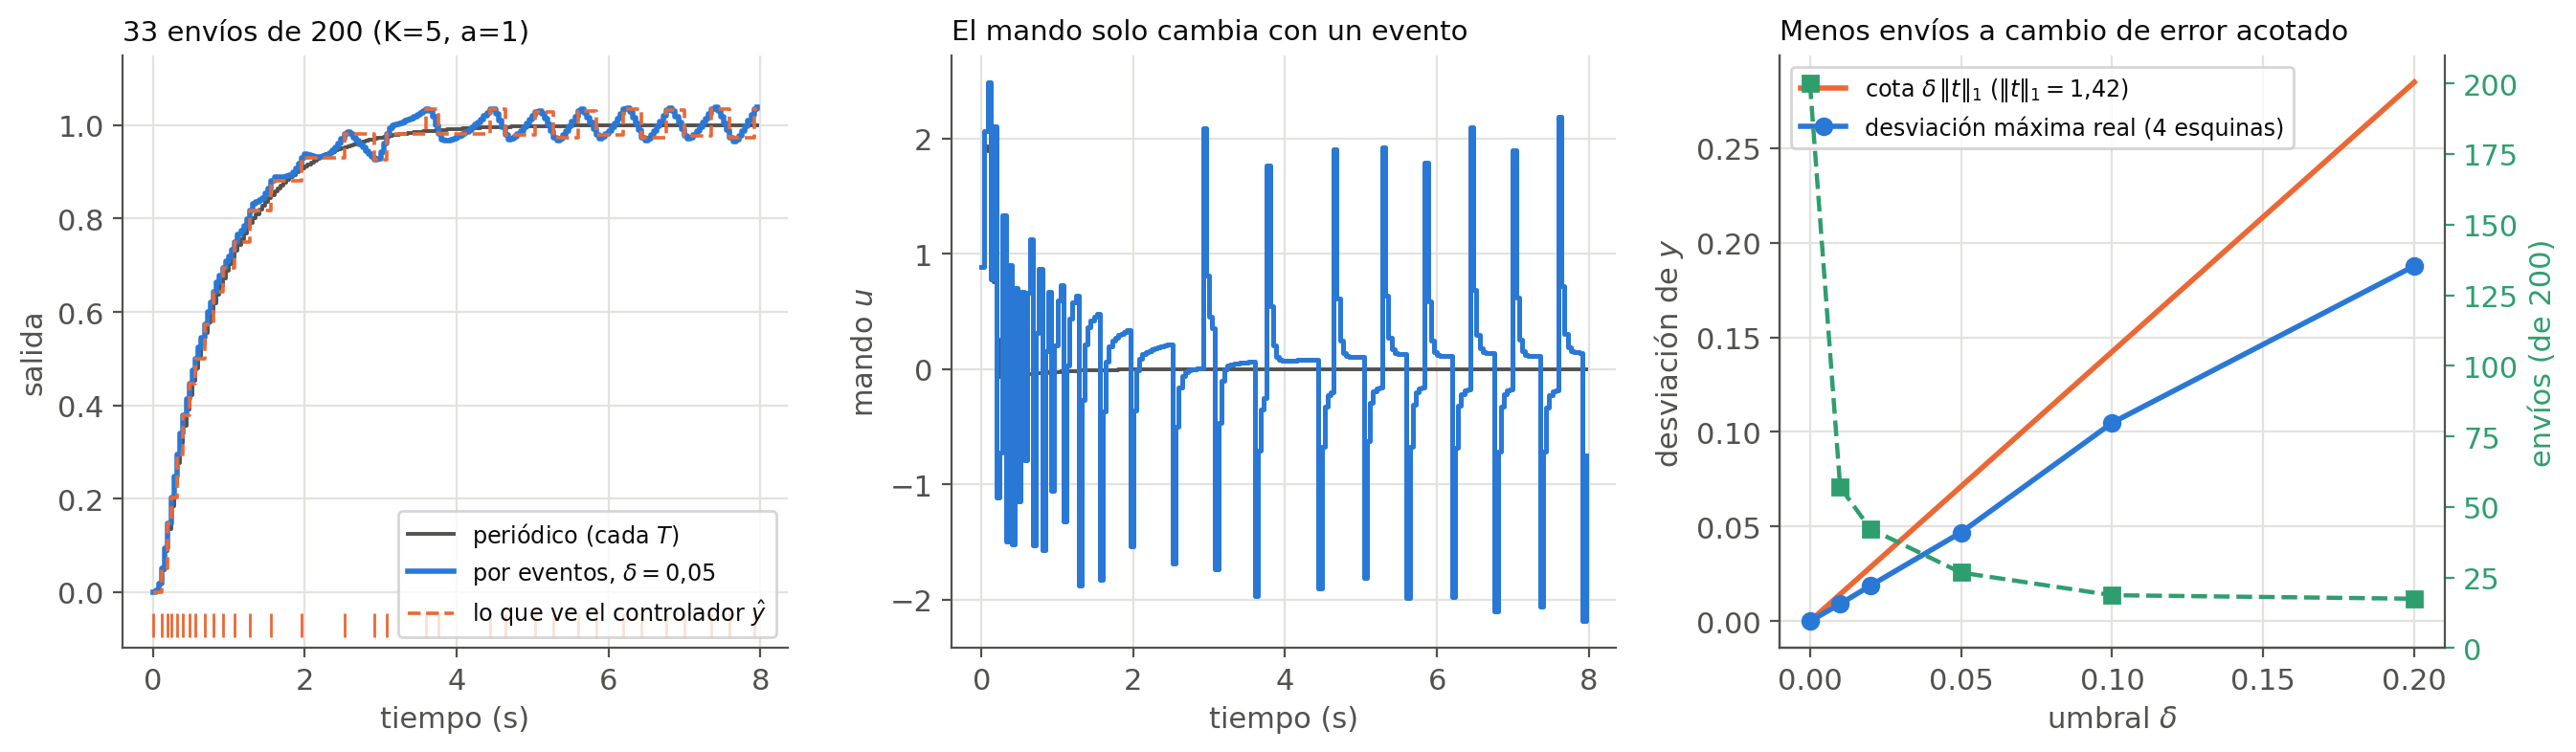
\includegraphics[width=0.97\textwidth]{fig/eventos.png}\\[0pt]
  \begin{itemize}
    \item Izquierda: con $\delta=0.05$ el lazo sigue a la referencia con \textbf{33 envíos de 200}. Cerca del final aparece una pequeña oscilación \textbf{dentro} de la banda $\pm\delta$: es un ciclo límite típico del disparo.
    \item Centro: el mando cambia a saltos de $\approx G(\infty)\,\delta=37.76\cdot0.05\approx1.9$. Un $\delta$ grande da mandos bruscos.
    \item Derecha: la desviación real (azul) queda siempre por debajo de la cota (naranja).
  \end{itemize}
\end{frame}

\begin{frame}{Cuánto se ahorra y cuánto se paga}
  \small
  \begin{center}
  \begin{tabular}{c|c|c|c}
    $\delta$ & envíos (de 200) & desviación máx. real & cota $1.42\,\delta$\\\hline
    0 & 200 & 0 & 0\\
    0.01 & 57 & 0.0091 & 0.0142\\
    0.02 & 42 & 0.0188 & 0.0285\\
    0.05 & 27 & 0.0469 & 0.0712\\
    0.10 & 19 & 0.1048 & 0.1424\\
    0.20 & 18 & 0.1877 & 0.2848
  \end{tabular}
  \end{center}
  \footnotesize
  Envíos: media de las cuatro esquinas de la familia; desviación: máximo de las cuatro. Referencia: escalón de $1$, 8 s.
  \begin{itemize}
    \item Con $\delta=0.01$ se envía \textbf{un 72\% menos} y el error extra es $<0.01$.
    \item A partir de $\delta\approx0.1$ casi no se ahorra más: quedan los envíos del transitorio.
  \end{itemize}
\end{frame}

\begin{frame}{Cómo elegir $\delta$ con una especificación}
  \footnotesize
  Es una especificación más, como las del paso 12:
  \begin{block}{Receta}
    Si la desviación admisible de la salida es $\Delta_y$, entonces
    \[ \delta\le\frac{\Delta_y}{\|t\|_1}. \]
    Si hay límite de mando por evento $\Delta_u$, también $\delta\le\Delta_u/G(\infty)$ (aquí $G(\infty)=37.76$).
  \end{block}
  \begin{itemize}
    \item $\|t\|_1$ se calcula una vez con las esquinas de la familia (o una rejilla densa).
    \item Un $\delta$ por debajo de la resolución del sensor no ahorra nada: no tiene sentido.
    \item En QFT, $\delta$ \textbf{no cambia} el diseño de $G$: solo añade una cota en la salida.
  \end{itemize}
  \begin{exampleblock}{Ejemplo}
    $\Delta_y=0.02\Rightarrow\delta\le0.02/1.42=0.014$. Con $\Delta_u=1$: $\delta\le1/37.76=0.026$. Manda el más restrictivo: $0.014$.
  \end{exampleblock}
\end{frame}

\begin{frame}{Umbral relativo: ahora sí cambia el diseño}
  \small
  Un umbral \textbf{proporcional} $|y_k-\hat y|\le\sigma\,|y_k|$ da $\hat y=(1+\Delta)\,y$ con $|\Delta|\le\sigma$.
  \begin{itemize}
    \item Es una \textbf{incertidumbre multiplicativa} en el sensor, no un ruido: afecta al lazo, $L\to L\,(1+\Delta)$.
    \item En QFT se mete en la familia: cada template se ensancha a un disco de radio $\sigma$ alrededor de cada punto (paso 12, incertidumbre no paramétrica).
    \item Estabilidad robusta por ganancia pequeña: $\sigma\,\max|T|<1$. Con $\max|T|=1.198$:
    \[ \sigma<\frac{1}{1.198}=0.83. \]
  \end{itemize}
  \begin{alertblock}{Pero estabilidad no es especificación}
    $\sigma<0.83$ asegura \textbf{estabilidad}. Mantener $|T|\le1.58$ dB y el seguimiento exige mucho menos.
  \end{alertblock}
\end{frame}

\begin{frame}{El diseño del paso 12 no aguanta ni $\sigma=0.05$}
  \footnotesize
  \centering
  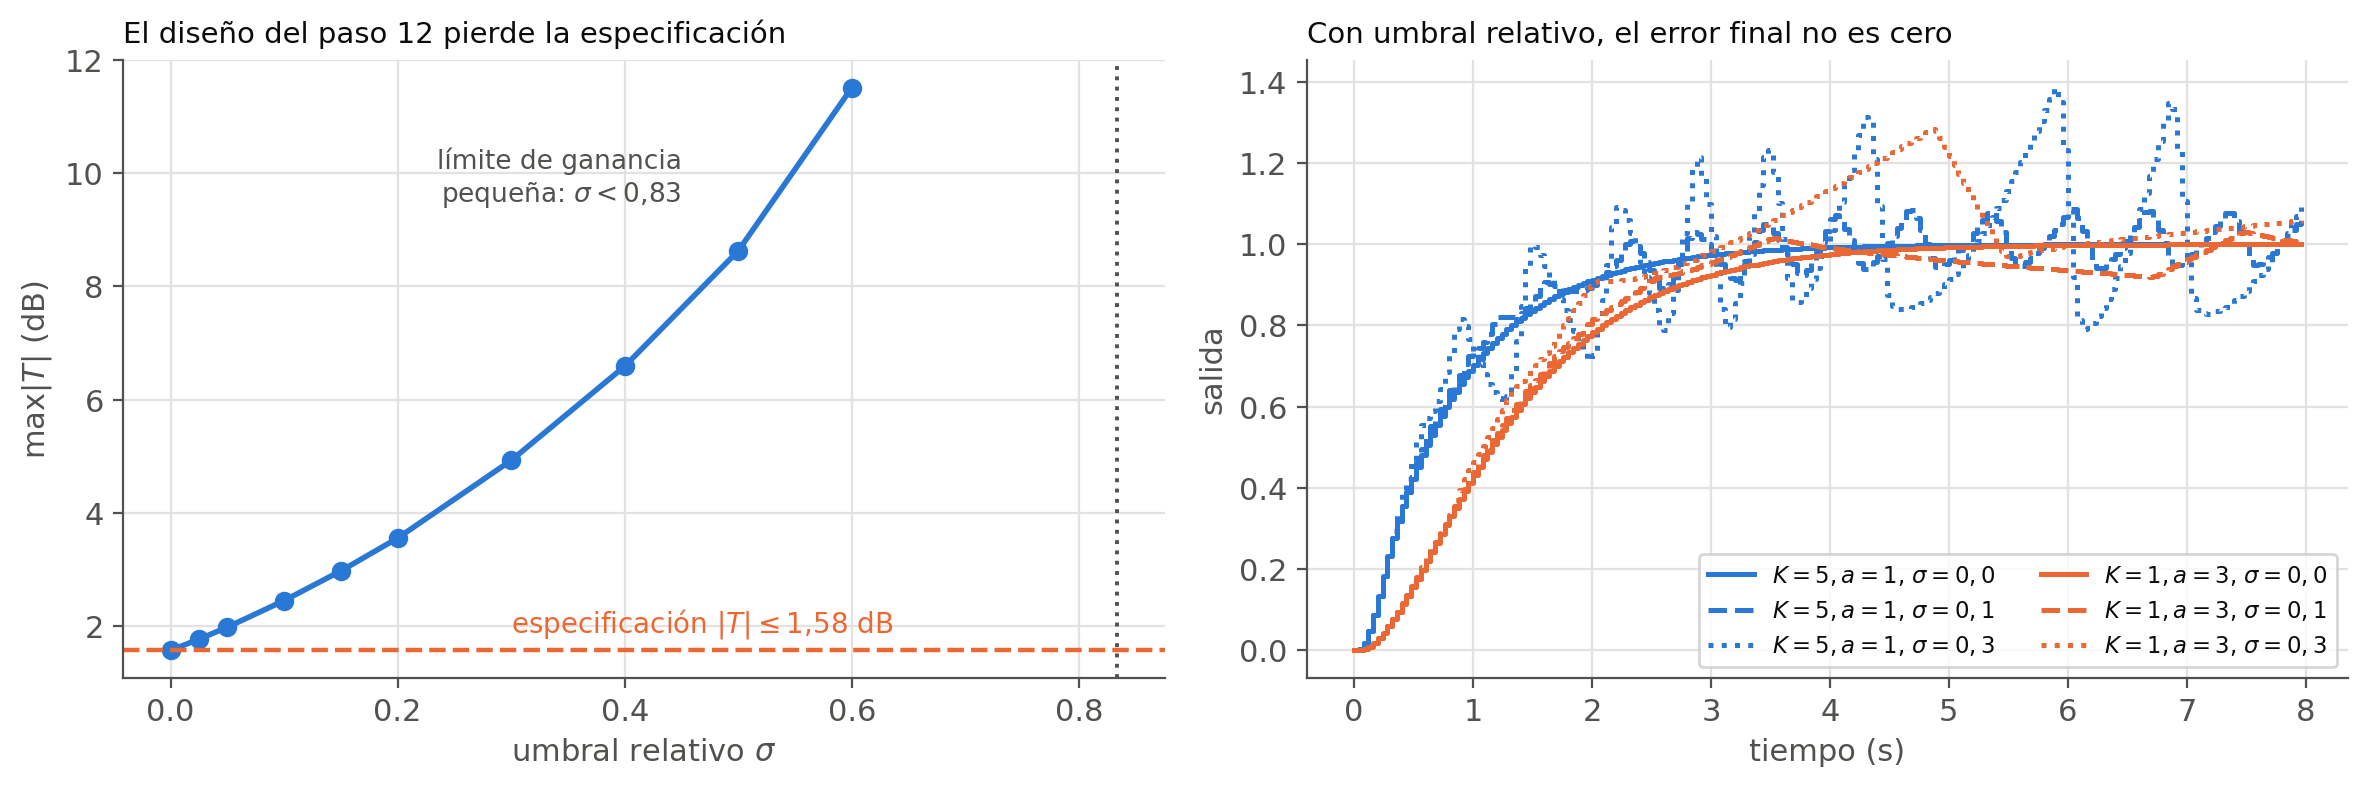
\includegraphics[width=0.92\textwidth]{fig/relativo.png}\\[2pt]
  \begin{itemize}
    \item $\max|T|$ sube de $1.57$ dB a $1.82$ dB con $\sigma=0.05$ y a $2.23$ dB con $\sigma=0.1$. El diseño del paso 12 tenía un margen de $0.02$ dB: \textbf{se gastó entero}.
    \item Para admitir $\sigma$ hay que \textbf{rediseñar} con la familia ensanchada (bounds más duros, más ganancia o menos ancho de banda).
    \item Con umbral relativo el error final \textbf{no} es cero: se queda dentro de $\pm\sigma\,y$ (a la derecha, $1.07$ con $\sigma=0.1$ y $K=5$, $a=1$).
  \end{itemize}
\end{frame}

\begin{frame}{Umbral mixto y tiempo máximo sin envío}
  \footnotesize
  \begin{columns}[T]
  \begin{column}{0.48\textwidth}
    \textbf{Umbral mixto} $|y_k-\hat y|>\delta+\sigma|y_k|$
    \begin{itemize}
      \item $\delta$ domina cerca de $0$: no se envía por ruido pequeño.
      \item $\sigma$ domina con señales grandes: ahorra en el transitorio.
      \item Se trata como la suma de las dos cosas: cota de ruido ($\delta$) más incertidumbre ($\sigma$).
    \end{itemize}
    \vspace{3pt}
    \textbf{Latido (\emph{heartbeat})}: si en $N$ muestras no ha habido evento, se envía igual.
    \begin{itemize}
      \item Con planta integradora y sin perturbación el silencio puede ser \textbf{largo}: aquí hasta $2.1$ s.
      \item El latido detecta un fallo del enlace y limita el peor retardo.
    \end{itemize}
  \end{column}
  \begin{column}{0.5\textwidth}
    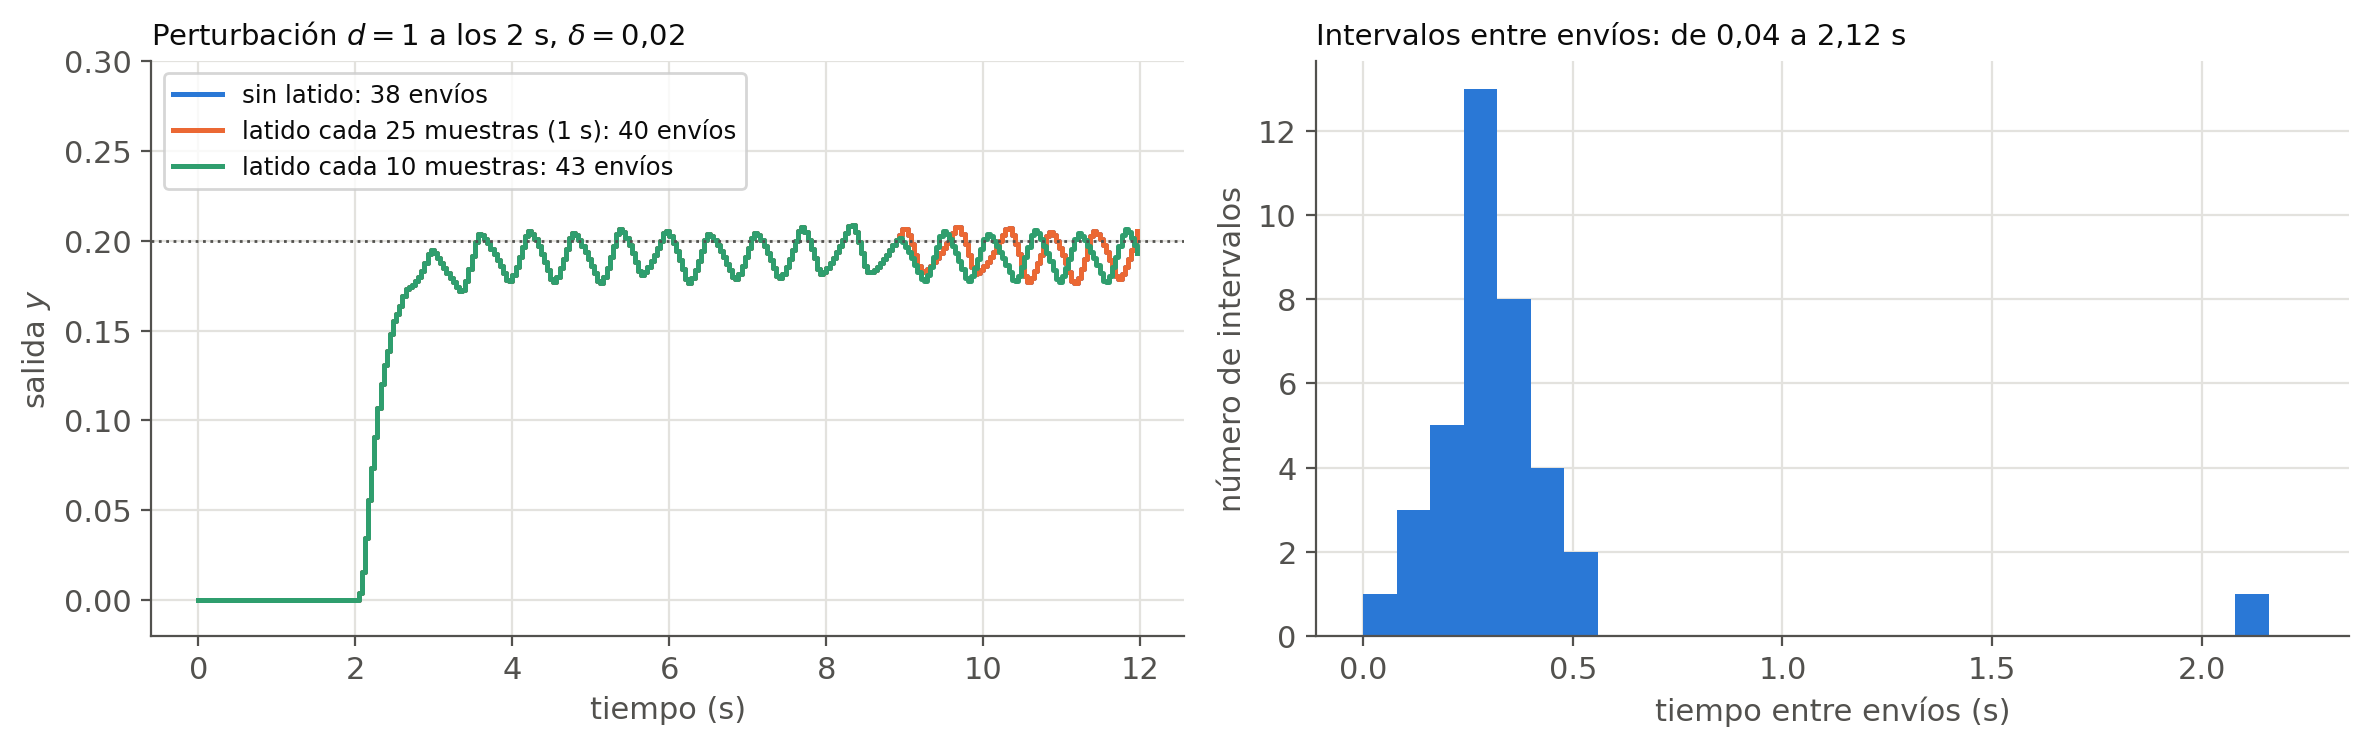
\includegraphics[width=\textwidth]{fig/latido.png}
    \vspace{2pt}\\
    Un latido de 25 o 10 muestras casi no cambia nada: la perturbación se detecta por evento, no por latido.
  \end{column}
  \end{columns}
\end{frame}

\begin{frame}{Qué dice QFT y qué no}
  \small
  \begin{columns}[T]
  \begin{column}{0.49\textwidth}
    \begin{block}{Lo cubre QFT}
      \begin{itemize}
        \item $\delta$ constante: ruido de medida acotado, cota $\delta\|t\|_1$.
        \item $\sigma$ relativo: incertidumbre multiplicativa en la familia.
        \item Estabilidad de la \textbf{familia} con $L(1+\Delta)$.
      \end{itemize}
    \end{block}
  \end{column}
  \begin{column}{0.49\textwidth}
    \begin{alertblock}{Lo que QFT no ve}
      \begin{itemize}
        \item El disparador es \textbf{no lineal}: los ciclos límite no salen del análisis frecuencial.
        \item El cumplimiento del seguimiento (banda $T_L$--$T_U$) es en régimen lineal; con $\delta$ grande se rompe.
        \item Retardos y pérdidas de paquetes: son otro tipo de incertidumbre.
      \end{itemize}
    \end{alertblock}
  \end{column}
  \end{columns}
  \vspace{4pt}
  Por eso se \textbf{simula} siempre el lazo con el disparador (como en la figura) tras diseñar.
\end{frame}

\begin{frame}{Resumen}
  \small
  \begin{itemize}
    \item Muestrear por eventos con periodo base $T$ = mirar cada $T$, enviar solo si $|y_k-\hat y|>\delta$.
    \item Umbral absoluto $\Rightarrow$ ruido de medida acotado: $|\Delta y|\le\delta\|t\|_1$. El diseño de $G$ no cambia.
    \item Umbral relativo $\Rightarrow$ incertidumbre multiplicativa $\sigma$: entra en la familia y gasta margen.
    \item Ahorro típico: $\delta=0.01$ da un \textbf{72\%} menos de envíos con error extra $<0.01$.
    \item Hay que simular el disparador: ciclos límite, mandos a saltos de $\approx G(\infty)\delta$.
  \end{itemize}
  \begin{block}{Ejercicio}
    (1) Con $\Delta_y=0.05$, ¿qué $\delta$ garantiza la cota? (2) Con $\delta=0.05$, ¿de cuánto es cada salto del mando? (3) ¿Por qué $\sigma=0.05$ ya incumple $|T|\le1.58$ dB?
  \end{block}
\end{frame}

\appendix
\begin{frame}{Solución del ejercicio}
  \footnotesize
  \textbf{1.} $\delta\le0.05/1.42=0.035$. En la tabla, $\delta=0.05$ da una desviación real $0.047$ (por debajo de $0.05$), pero la \textbf{garantía} solo llega hasta $0.035$.\\[3pt]
  \textbf{2.} El salto es $G(\infty)\cdot\delta=37.76\cdot0.05\approx1.9$ (el término $-34.03\,z^{-1}$ lo compensa en régimen, no en el primer instante).\\[3pt]
  \textbf{3.} El diseño tenía margen $0.02$ dB sobre la especificación. Con $\sigma=0.05$ el peor $|T|$ sube de $1.57$ a $1.82$ dB (calculado en 24 fases del disco $\Delta=\sigma e^{j\phi}$, sobre una rejilla de la familia).
\end{frame}
\end{document}
